\chapter{Zenbakizko integratzaile sinplektikoak}

\section{Sarrera}

Lan honen xede nagusia, N-gorputzeko sistema grabitazionalaren problemen zenbakizko integraziorako algoritmoak garatzea edo daudenak hobetzea da. Era horretako problemen artean, eguzki-sistemaren epe luzeko integraziorako inplementazioak aztertuko ditugu \cite{Kholshevnikov2007,Brumberg2013} . Gaur egun, era horretako integrazioetarako hainbat zenbakizko metodo erabiltzen dira, bereziki bere izaera Hamiltondarra mantentzen duten metodo sinplektikoak \cite{Eggl2010,Saha1992,Farres2013}. Metodo horien artean, gehien erabiltzen direnak izaera esplizituko algoritmoak diren arren, metodo inplizituak, modu egokian inplementatuz gero, hauek baino eraginkorragoak izan daitezke. Zenbakizko integraziorako Gauss metodo inplizituaren inplementazio eraginkorra aztertuko dugu.   

Atal honen lehen zatian, zenbakizko integrazio-metodoen inguruko oinarrizko definizioak eta kontzeptuak azalduko ditugu. 
Jarraian, sistema Hamiltondarrak zer diren eta halakoak integratzeko erabiltzen diren metodo sinplektikoak azalduko ditugu. Ondoren, zenbakizko integratzaile sinplektiko nagusienak aztertuko ditugu: alde batetik, Runge-Kutta metodo sinplektikoak (inplizituak); eta bestetik, konposizio eta splitting metodo sinplektikoak (esplizituak).

\section{Zenbakizko integrazio metodoak}

\subsection{Oinarrizko kontzeptuak}

Ekuazio diferentzial arruntak, egoera-aldaketak dituzten problemen azterketarako eredu matematikoak dira \cite{Hairer2015}. Zientziaren eta ingeniaritzaren arlo askotan azaltzen zaizkigu: planeten mugimenduen ereduetan (astronomia), erreakzio kimikoen formulazioetan, molekulen dinamiken simulazioetan, zirkuitu elektronikoen diseinuan, populazio-hazkunde eta interakzioetan (biologian), ekonomia azterketetan \ldots  

Ekuazio diferentzial arrunta, $y(t)$ soluzio ezezagunaren eta bere $\dot{y}(t)$ deribatuaren arteko erlazioa da. $t$ aldagaiak, maiz denbora adierazten du eta $y(t) \in \mathbb{R}^{d}$ soluzio bektorea da. Deribatua, modu esplizituan denboraren eta egoeraren arabera  adieraz daitekeenean, era honetako ekuazioak ditugu,
\begin{equation}
 \label{eq:201}
\dot{y}(t)=f(t,y(t)). 
\end{equation} 
$\dot{y}$ notazioa erabiliko dugu $dy/dt$ adierazteko.

Ekuazio diferentzial arruntetarako hasierako baliodun problemetan,  $y(t_0)=y_0 \in \mathbb{R}^d$ hasierako balio bat finkatuz, eta $f(t,y)$ funtzioa, $f: \mathbb{R}^{d+1} \longrightarrow \mathbb{R}^d, \ \ t_0$ ingurunean diferentziagarria bada, orduan hasierako baliodun problemaren soluzioa existitzen da eta bakarra da \cite{Hairer2006},
\begin{equation}
 \label{eq:ivp}
\dot{y}(t)=f(t,y(t)), \ \ \ y(t_0)=y_0.
\end{equation} 

(\ref{eq:ivp}) ekuazio-sistema bektoriala, modu eskalarrean idatziko dugu orokorrean erabiliko dugun notazioa argitzeko:
\begin{align*}
&\dot{y}^1(t)=f^1(t,(y^1(t),y^2(t),\ldots,y^d(t))), \\
&\dot{y}^2(t)=f^2(t,(y^1(t),y^2(t),\ldots,y^d(t))), \\
&\ldots\ \ ,\\
&\dot{y}^d(t)=f^d(t,(y^1(t),y^2(t),\ldots,y^d(t))),  \\
& y(t_0)=(y_{0}^1,\ y_{0}^2,\ \ldots \ , \ y_{0}^d).
\end{align*}


Oso problema gutxitarako aurki daiteke ekuazio diferentzial arrunten soluzio analitikoa (funtzio ezagunen araberako soluzio zehatza) eta beraz, ia problema gehienak zenbakizko integrazio metodoen bidez ebazten dira.
Zenbakizko integrazioetan, soluzioaren hurbilpena,
\begin{align*}
 y_n \approx y(t_n), \ t_n=t_{n-1}+h_n, \ n=1,2,\dots
\end{align*}
une diskretu konkretuetarako, zehaztutako tarte batean ($t_0\le t \le t_f$) lortuko da. Zenbakizko soluzioa, sekuentzialki urratsez-urrats kalkulatzen da eta lortutako balio  multzoak $(t_0,y_0),(t_1,y_1),\dots,(t_f,y_f)$ zenbakizko soluzioa definitzen du.   

Ekuazio diferentziala beti \emph{sistema autonomo} moduan, hau da, denborarekiko independenteki, idatz daiteke. Hori horrela izanik, notazioa sinplifikatzeko era honetako hasierako baliodun problemak kontsideratuko ditugu,   
\begin{equation}
\label{eq:autonomo}
\dot{y}(t)=f(y(t)),\ \ \ y(t_0)=y_0.
\end{equation}

\subsubsection*{Definizioak}  
Jarraian zenbakizko integrazioen metodoen oinarrizko kontzeptuak eta notazioa finkatuko ditugu \cite{Corless2013,Hairer2006}.
\begin{enumerate}
\item Fluxua

Fase-espazioko edozein $y_0$ baliori, $y(t_0)=y_0$ hasierako balioa duen $y(t)$ soluzioa esleitzen dion funtzioari fluxua deitzen zaio. Izendatzeko $\varphi_h$ notazioa erabiliko dugu,
\begin{equation*}
\label{eq:fluxua}
\varphi_h(y_0)=y(t_0+h) \ \ \mbox{baldin}  \ \  y(t_0)=y_0.
\end{equation*}

\item Zenbakizko diskretizazioa

$y_{n}$ balioa emanda, $y_{n+1}\approx y(t_{n+1})$ soluzioaren hurbilpena kalkulatzeko formulari \emph{zenbakizko fluxua} deritzogu. Honako notazioa erabiliko dugu,
\begin{equation}
\label{eq:204}
y_{n+1}=\phi_h(y_{n}).
\end{equation}

\item Metodoaren ordena

\begin{enumerate}
\item Errore lokala deritzo,  $y(t_0)=y_0$ soluzio zehatzetik abiatuta, integrazio metodoaren urrats bat eman ondoren lortutako zenbakizko soluzioak benetako soluzioarekiko duen aldeari.
\begin{equation*}
\label{eq:le}
\delta(y,h)=\varphi_h(y)-\phi_h(y).
\end{equation*}   


\item Errore globala esaten zaio, zenbakizko soluzioaren $t_0$ hasierako unetik $t_k$ unera hainbat urrats emanez integratu ondoren $y(t_k)$ soluzioarekiko duen aldeari,
\begin{equation*}
 \label{eq:ge}
E(t_k)=y_k-y(t_k).
\end{equation*}  

\item Metodoaren ordena. $h$ urrats luzera finkoko $\phi$ metodoa $p$ ordenakoa dela esaten da, $E(t)$ errore globala $\mathcal{O}(h^{p})$ ordenakoa bada  $h \rightarrow 0$,
\begin{equation*} 
\label{eq:metordena}
\|y_k-y(t_k)\|=\mathcal{O}(h^{p}), \ \ h \rightarrow 0.
\end{equation*} 
Metodoaren ordena $\mathcal{O}(h^p)$ bada, errore lokala $\mathcal{O}(h^{p+1})$ da.

\end{enumerate}

\item  Metodo simetrikoak

Urrats bakarreko $\phi_h$ metodoa simetrikoa da, honako baldintza betetzen badu,
\begin{equation*}
\phi_h \circ \phi_{-h}=id,  \ \ \text{edo} \ \ \phi_h=\phi_{-h}^{-1}.
\end{equation*}


\end{enumerate}


\subsubsection*{Euler-en metodo esplizitua}

Euler-ek $1768.$ urtean proposatutako zenbakizko metodoa da. Hasierako balio bat emanda $(t_n,y_n)$ eta $h_n>0$ urrats txikirako, $t_{n+1}=t_{n}+h_{n}$ uneko hurbilpena $y_ {n+1} \approx y(t_{n+1})$ era honetan kalkulatuko dugu,  
\begin{equation*}
 \label{eq:202a}
y_{n+1}=y_{n}+h_n f(t_n,y_n).
\end{equation*}
Oinarrizko metodo esplizitua da eta urratsa emateko dagoen konputazio konplexutasun bakarra $f$ funtzioaren ebaluazio da. Lehen ordenako metodoa da,
\begin{equation*}
\|y_n-y(t_n)\| \leqslant C h, \ C \in \mathbb{R}
\end{equation*}
eta beraz, doitasuna bikoizteko, lan konputazionala bikoiztu behar dugu. Ikusiko dugunez, ordena altuagoko metodoekin doitasun handiagoa lortuko dugu, lan konputazional gutxiagorekin. 

\subsubsection*{Euler-en metodo inplizitua}

Euler-ek proposatutako beste metodo honek, $y_{n+1}$ hurbilketa, inplizituki definitzen den funtsezko ezaugarria du. $f$ funtzioaren argumentua, aurreko hurbilpenaren ordez hurbilpen berria hartuz definitzen da,
\begin{equation*}
 \label{eq:202b}
y_{n+1}=y_{n}+h_n \ f(t_{n+1},y_{n+1}).
\end{equation*}
Urratsa emateko, ekuazio-sistema ez-linealaren soluzioa askatu behar da. Horretarako, iterazio metodo bat aplikatu behar da.

\subsubsection*{Iterazio metodoak}

Ekuazio-sistema ez-linealen soluzioa askatzeko bi iterazio metodo azalduko ditugu.

\begin{enumerate}

\item Puntu-finkoaren iterazioa

$x=f(x)$ ekuazioa, non $f: {\mathbb{R}}^n  \longrightarrow {\mathbb{R}}^n$ eta  $x^{[0]} \in \mathbb{R}^n$ soluzioaren hasierako hurbilpen bat emanda, puntu-finkoaren iterazioa era honetan definitzen da,
\begin{equation*}
 x^{[k+1]}=f(x^{[k]}) \, \ \ \ \ \ k=1,2,\dots
\end{equation*}
Iterazioak $x^{\ast}$ soluzioarengana konbergitu dezake.

Eta  Euler metodo inplizituaren ekuazio ez-lineala askatzeko, $y_{n+1}^{[0]}$ balioa finkatuta, puntu-finkoaren iterazioa era honetan aplikatuko dugu, 
\begin{equation*}
y_{n+1}^{[k+1]}=y_{n}+h_n \ f(t_{n+1},y_{n+1}^{[k]}), \ \ \ \ \ k=1,2,\dots
\end{equation*}  

\item Newtonen iterazioa

Demagun $f(x)=0$ ekuazioa askatu behar dugula, hau da, $f(x)$-ren erro baten bila gabiltzala,
 non $f: \  {\mathbb{R}}^n \ \longrightarrow {\mathbb{R}}^n$ eta  $x^{[0]} \in \mathbb{R}^n$ soluzioaren hasierako hurbilpen bat den, Newtonen iterazioa era honetan definitzen da,
\begin{align*}
&k=1,2,\dots \\
&\Delta x^{[k]} \ J(x^{[k]})=-f(x^{[k]}), \\
&x^{[k+1]}=x^{[k]}+\Delta x^{[k]} 
\end{align*}
non $J(x)=\frac{\partial f}{\partial x} (x)$ den.

\end{enumerate}

Urratsaren konputazioaren konplexutasuna metodo esplizituan baino nabarmen handiagoa da: metodo honetan, iterazio bakoitzean Jacobiarra balioztatu, ekuazio-sistema lineala askatu eta $f$ funtzioaren ebaluazioa kalkulatu behar dira.

Iterazio metodoaren konbergentzia abiadura. $\{x^{[0]},x^{[1]},\dots,x^{[k]}\}$, $x^{\ast}$ soluziorantz konbergitzen duen bektore seriea bada, errorea $e^{[n]}=x^{[*]}-x^{[n]}, \ n=1,2,\dots$ izendatuko dugu. Konbergentzia $p$ ordenakoa dela esaten dugu honakoa betetzen dada,
\begin{equation*}
\lim\limits_{n\rightarrow \inf} \frac{\|e^{[n+1]}\|}{\|e^{[n]}\|^p}= C \ne 0.
\end{equation*}

Puntu-finkoaren iterazioak konbergentzia lineala ($p=1$) du, Newtonen iterazioak, berriz, koadratikoa ($p=2$). Konbergentzia koadratikoa izatea oso interesgarria da, iterazio bakoitzean soluzioaren digitu hamartar zuzenen kopurua bikoizten dugulako. Konbergentzia linealean, ordea, iterazio bakoitzean digitu hamartar kopuru finkoa hobetzen dugu. 
  
\subsubsection*{Problema zurruna}

Urrats baten konputazio-kostua handiagoa izan arren, problema batzuetan metodo inplizituak esplizituak aplikatzea baino egokiago izan daiteke, eta hori erakusteko Germund Dahlquist-en ($1963$) adibidea azalduko dugu,
\begin{equation}
 \label{eq:202c}
\dot y=\lambda y,
\end{equation} 
non $\lambda$ balio absolutuan handia eta negatiboa den. Problema honen soluzio analitikoa ezaguna da, $y(t)=e^{(t-t_0)\lambda}$, eta $t \rightarrow \infty$ doanean, soluzioa zerorantz gerturatzen da. Metodo inplizituaren bidezko zenbakizko soluzioa zerorantz gerturatzen da $h>0$ guztietarako,
\begin{equation*}
y_n^{impl}=(1-h\lambda)^{-n} y_0,
\end{equation*}    
eta aldiz, metodo esplizituaren bidezkoa,
\begin{equation*}
y_n^{expl}=(1+h\lambda)^{n} y_0,
\end{equation*}    
zerorantz gerturatuko da soilik $h$ oso balio txikitarako, non $|1+h\lambda|<1$ izan behar duen. Beraz, problema honetan $\lambda$ balio absolutuan handia  eta negatiboa definitu dugunez (adibidez $\lambda=-10^{10}$), Euler esplizituan $h$ urrats tamaina oso txikia erabili behar dugu.    

Euler inplizitua, Euler esplizitua baino eraginkorragoa den ekuazio diferentzialei, problema \emph{zurrunak} (\emph{stiff}) esaten zaie \cite{Hairer2006}. Problema \emph{zurrunen} artean problema garrantzitsuak ditugu, esaterako eskala anitzeko sistemak. 
 

\subsection{Sistema-Hamiltondarrak}

 
Hamiltondar sistemak \cite{SSerna2015}, ekuazio diferentzial mota garrantzitsu bat dira. $H(q,p)$ funtzio leunari dagokion \emph{Hamiltondar sistema} osatzen duten $2d$ ekuazio diferentzialak, era honetan definitzen dira,
\begin{align*}
\label{eq:212}
\frac{d {p}^i}{dt} & =-\frac{\partial H (q,p)}{\partial q^i} , \\
\frac{d {q}^i}{dt} & =+\frac{\partial H (q,p)}{\partial p^i} , \ \ \ \ i=1,\dots,d,
\end{align*}
non $H: {\mathbb{R}}^{2d} \ \longrightarrow {\mathbb{R}}$  den eta  $q=[q^1, \dots , q^d]^T$, $p=[p^1, \dots , p^d]^T$  domeinuaren aldagaiak diren. Egoera aldagaien bektoreen $d$ dimentsioari, sistemaren \emph{askatasun maila} esaten zaio. $H(q,p)$ funtzioari \emph{Hamiltondarra} deritzo, eta sistemaren energia adierazten du. Energia, integrazioan zehar konstante mantentzen da,
\begin{equation*}
\label{eq:212b}
H(q(t),p(t))=K, \ K \in \mathbb{R}.
\end{equation*}

Beste notazio laburtu hau ere erabili ohi da,
\begin{equation*}
 \label{eq:213}
\dot{y}=J^{-1}\triangledown H(y),
\end{equation*}

non $y=(q,p)$, $\triangledown H=(\partial H/\partial q^1,\dots,\partial H/\partial q^d; \partial H/\partial p^1,\dots,\partial H/\partial p^d)$ eta

\begin{equation*}
 J=\left(\begin{array}{cc}
   \ 0_{dxd} & \ I_{dxd} \\
    -I_{dxd} & \ 0_{dxd} \\
\end{array}\right), \ \ \ 
I_{d \times d}=\left(\begin{array}{cccc}
   \ 1       & 0      & \cdots & 0 \\
   \ 0       & 1      & \cdots & 0 \\
   \ \vdots  & \vdots & \ddots & \vdots \\
   \ 0       & 0 & \cdots & 1 \\
\end{array}\right)  
\end{equation*}


\paragraph*{Hamiltondar banagarriak.} Sistema dinamikoen Hamiltondarrak, maiz egitura berezia du,
\begin{equation*}
H({q},{p})=T(p)+U({q}).
\end{equation*} 

Horien artean, \emph{bigarren ordenako} ekuazio diferentzialak aipatu behar ditugu. Hauek Hamiltondar banagarrien kasu partikular bat dira. Bere Hamiltondarra  
\begin{equation*}
H(\mathbf(q,p)=\frac{1}{2}p^Tp +U(q),
\end{equation*}
da eta dagokien ekuazio diferentzialak hauek dira,
\begin{equation}
\label{eq:biorden}
\dot{p}=-\frac{\partial U(q)}{\partial q}, \ \ \dot{q}=p. 
\end{equation}

\paragraph*{Adibidea.}
\emph{Kepler problema} \cite{Hairer2006}. Planoan elkar erakartzen diren bi gorputzen mugimendua adierazten duen problema da (adibidez eguzkia eta planeta bat). Gorputz baten kokapena koordenatu sistemaren jatorria kontsideratuko dugu eta beste gorputzaren kokapenaren koordenatuak $q=(q_1,q_2)$ izendatuko ditugu. $p=(p_1,p_2)$ momentuak dira. 

Funtzio Hamiltondarra hauxe da,
\begin{equation*}
H(q_1,q_2,p_1,p_2)=\frac{1}{2}(p_1^2+p_2^2)-\frac{1}{\sqrt{q_1^2+q_2^2}}.
\end{equation*}

Dagozkion ekuazio diferentzialak,
\begin{align*}
\dot{p}_1 &= -\frac{q_1}{(q_1^2+q_2^2)^{3/2}}, \ \, \dot{p}_2= -\frac{q_2}{(q_1^2+q_2^2)^{3/2}}, \\
\dot{q}_i &=p_i, \ \ \ \ \ i=1,2.
\end{align*}

Planetaren mugimendua orbita eliptiko bat da. Honako hasierako balioei dagokien soluzioa zehatza,
\begin{equation*}
q_1(0)=1-e, \ q_2(0)=0, \ p_1(0)=0, \ p_2(0)=\sqrt{ \frac{1+e}{1-e}}, 
\end{equation*}
$e$ ezentrizidadea ($0\le e < 1$)  eta $P=2\pi$ periodoa duen elipsea da. 

\paragraph*{Hamiltondar perturbatuak.} Hamiltondar perturbatuak, honako egitura duten sistemak ditugu,
\begin{equation*}
H=H_A+\epsilon H_B \ \  \text{non} \ \ |H_B|\ll |H_A|.
\end{equation*}

\paragraph*{Adibidea.} Eguzki-sistemaren probleman \cite{Saha1992,Wisdom2006}, Hamiltondarra modu honetan bana daiteke $H=H_k+H_I$, non alde nagusia $H_K$ planeta bakoitzaren eguzkiaren inguruko mugimendu Kepleriarrari dagokion eta $H_I$, aldiz, planeten arteko interakzioek eragiten duten perturbazio txikiari.   

\subsection{Metodo sinplektikoak}

Hamiltondar sistemen problemetarako Euler esplizitua eta Euler inplizitua ez dira zenbakizko metodo egokiak, ez baitute Hamiltondarra mantentzen. Problema hauen propietate geometrikoak mantentzen dituzten integratzaile bereziak beharrezkoak dira \cite{JMSanz-Serna1994,SSerna2015b}. Integratzaile hauek, metodo sinplektikoak dira eta abantaila handiena, epe luzeko integrazioetan azaltzen dute.

Metodo sinplektikoen lehen aipamenak, $1950$ hamarkadan kokatu behar dira eta $1980$ hamarkadan, Feng Kang-ek metodo hauen azterketa sakona burutu zuen. Hastapenetako lan monografiko hau \cite{JMSanz-Serna1994} eta ondorengo, azalpen ulergarriak jasotzen dituzten \cite{Hairer2006} eta  \cite{Leimkuhler2004} lanak azpimarra daitezke.    

%\begin{figure}[h!]
%\centering
%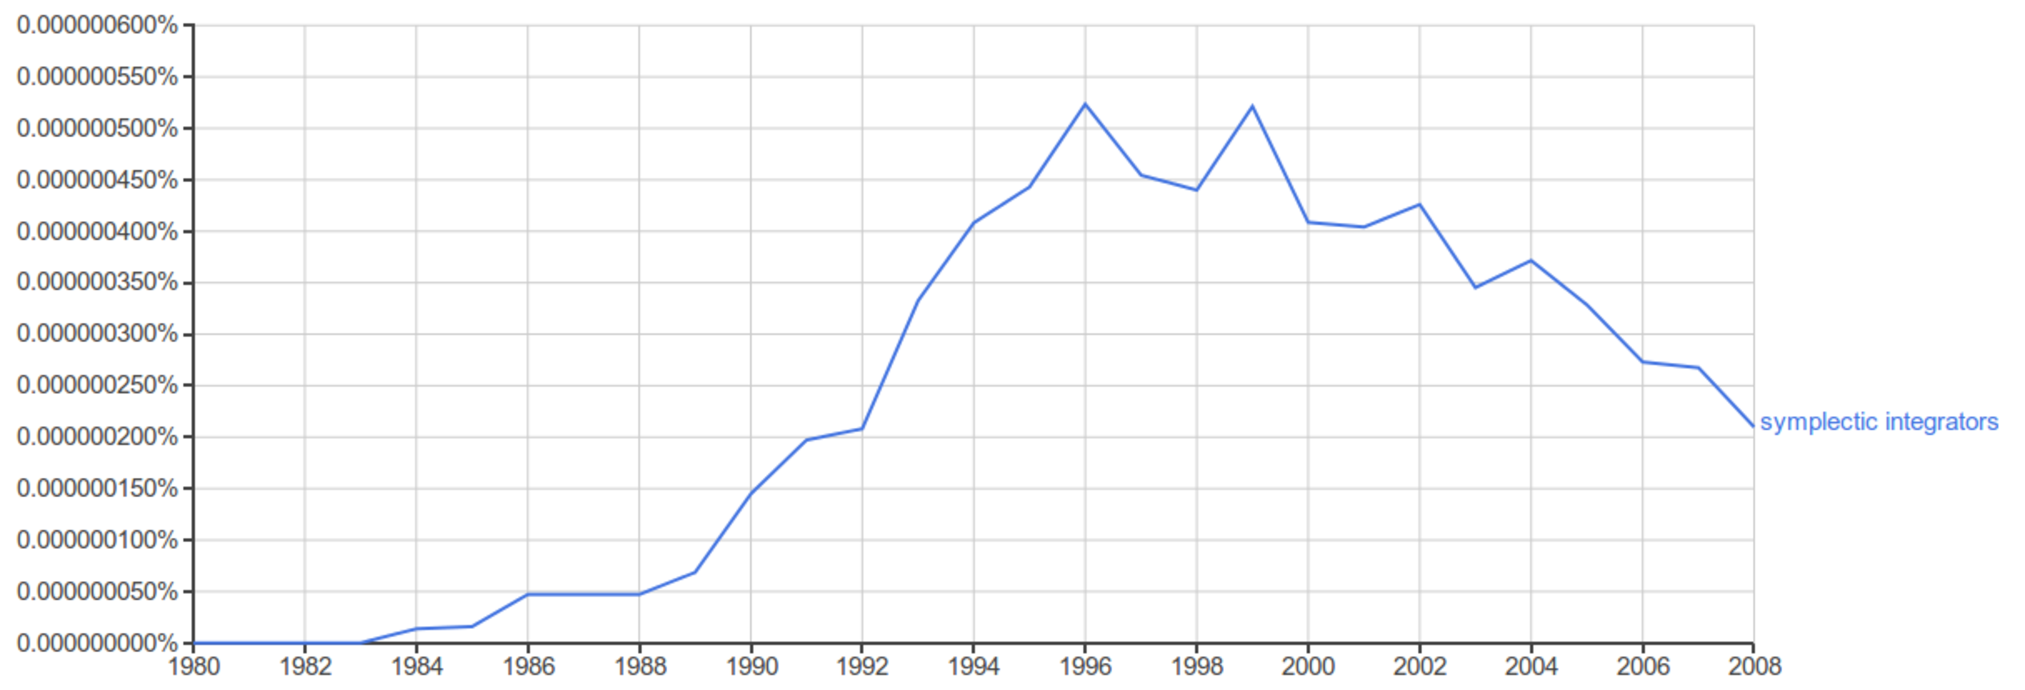
\includegraphics[width=1.0\textwidth]{NgramSymplectic}
%\caption{ \small Google-n ngram aplikazioan "symplectic integrators" gaiaren bilaketan, lortutako irudia.}
%\label{fig:NgramSymplectic}
%\end{figure}

\paragraph*{Adibidea.} Metodo sinplektikoen abantaila azaltzeko, penduluaren problema aukeratu dugu \cite{Hairer2015a}. Penduluaren problema (masa $m=1$, $l=1$ luzerako makila eta $g=1$ grabitazioa) $d=1$ askatasuneko sistema Hamiltondarra da:
\begin{equation}
H(q,p)= \frac{p^2}{2}- cos (q),
\end{equation}
%
eta ekuazio diferentzialak honakoak dira,
\begin{equation}
\label{eq:pendulua}
\dot{p}= -sin (q), \ \ \dot{q}=p.
\end{equation}

\ref{fig:pendulua}~irudian ikus daitekeenez, Euler esplizitu eta inplizituaren portaera kualitatiboki okerra da. Euler sinplektikoak  ordea, sistemaren energia kontserbatzen du, bere definizioa den \cite{Hairer2006}: 
\begin{align}
\label{eq:eulersin}
\begin{split}
p_{n+1} & =p_n-h \ \frac{\partial H }{\partial q} (p_{n+1},q_{n}), \\
q_{n+1} & =q_n+h \ \frac{\partial H}{\partial p} (p_{n+1},q_{n}).
\end{split}
\end{align}

\begin{figure}[h!]
\centering
\begin{tabular}{c c}
\subfloat[Pendulua.]{
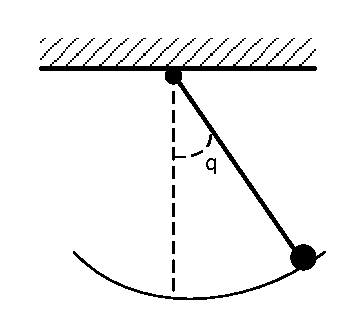
\includegraphics[width=.30\textwidth]{PenduluArrunta}
}
&
\subfloat[Integrazioa.]{
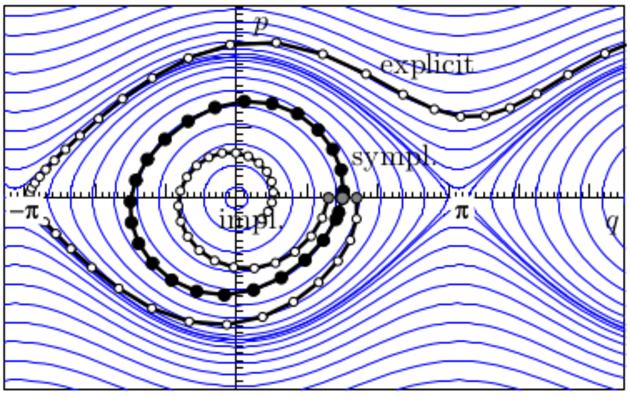
\includegraphics[width=.40\textwidth]{pcam-irudia}
}
\end{tabular}
\caption[Pendulu arrunta]{ \small Pendulu problemaren hiru zenbakizko metodoen zenbakizko soluzioak irudikatu ditugu. Hiruretan urrats luzera berdina $h=0.3$ baina bakoitza hasierako balio ezberdinarekin. Euler esplizitua $(p(0),q(0))=(0,1.7)$; Euler sinplektikoa $(p(0),q(0))=(0,1.5)$; Euler inplizitua $(p(0),q(0))=(0,1.3)$}
\label{fig:pendulua}
\end{figure}


Metodo sinplektikoak bi taldetan banatuko ditugu: metodo sinplektiko inplizituak eta  esplizituak. Lehenengo taldean,  Runge-Kutta metodo inplizituak (Gauss kolokazio metodoak) ditugu. Metodo hauek zenbakizko metodo estandarrak dira eta ekuazio diferentzial orokorrei aplika dakizkieke. Bigarren taldean, konposizioan eta splitting-ean oinarritutako metodoak ditugu. Azken talde honetako metodoak, bakarrik Hamiltondar sistemei aplika dakizkieke eta gainera, Hamiltondarrak banagarria izan behar du. Konposizio eta splitting metodoak oso eraginkorrak dira.   


\subsubsection*{Metodo sinplektikoen propietateak}

%Zuzenketa Joseba 04-05-2017
%Funtsezkoa da, integratzaile sinplektiko baten bidez lortutako $H$ Hamiltondar sistemaren zenbakizko soluzioa, perturbatutako beste %Hamiltondar $\widetilde{H}$ baten soluzio zehatza gisa ulertzea \cite{SSerna2015b}. Kontutan hartu behar da, zenbakizko integrazioak %eragiten dituen perturbazio hauek, sistema dinamiko baten $H$ Hamiltondar eredua eraikitzerakoan, hartzen  diren hurbilpenek edo datu ez %ziurrek eragiten duten baino errore maila txikiagoa suposatzen dutela.    
 
Integratzaile sinplektiko baten bidez sistema Hamiltondar baten soluzioa lortzen dugunean, ez dugu lortzen jatorrizko sistemaren soluzio zehatza, baina lortutako soluzio hori bera jatorrizko sistemaren perturbazio baten soluzio zehatza da \cite{SSerna2015b}. Alegia, lortutako soluzioa beste sistema Hamiltondar baten soluzio zehatza da.  

% Josebaren zuzenketa 06-05-2017: adibidea kendu
%\paragraph{Adibidea.}
%Demagun, askatasun maila bakarra duen sistema Hamiltondar banagarria $H=T(p)+V(q)$, Euler metodo sinplektikoaren (\ref{eq:eulersin}) bidez integratzen dugula.  $(p_n,q_n)$ zenbakizko soluzioak, integratu nahi dugun $S$ Hamiltondar sistemaren $(p(t_n),q(t_n))$ soluzio zehatza hurbiltzen du.  Modu honetan, benetako fluxua $\varphi_h^H$ eta zenbakizko integrazioa $\phi_h^H$ izendatzen baditugu,
%\begin{align*}
%&(p_{n+1},q_{n+1}) =\phi_h^H(p_n,q_n), \\
%&(p(t_{n+1}),q(t_{n+1})) =\varphi_h^H(p(t_n),q(t_n)), 
%\end{align*} 
%eta Euler sinplektikoa $p=1$ ordenako metodoa denez,
%\begin{equation*}
%\phi_h^H(p_n,q_n)-\varphi_h^H(p(t_n),q(t_n))= \mathcal{O}(h^2).
%\end{equation*}    

%Defini ahal daiteke beste $S_2$ Hamiltondar sistema bat, zeinekin Euler sinplektikoa bigarren ordenako den? Hau da, $(p_n,q_n)$ zenbakizko soluzioa, $S$ soluziotik baino gertuago dagoen $S_2$ sistema? 
%\begin{align*}
%\phi_h^{\widetilde{H}}(p_n,q_n)-\varphi_h^{\widetilde{H}}(p(t_n),q(t_n))= \mathcal{O}(h^3).
%\end{align*}

%Taylor seriea garatuz, lortuko dugu $S_2$ sistema  ($f=-\partial H/\partial q$, $g=\partial H/\partial p$),
%\begin{align*}
%\frac{d}{dt} p &= f(q)+ \frac{h}{2} g(p) f'(q),\\
%\frac{d}{dt} q &= g(p)- \frac{h}{2} g'(p) f(q),
%\end{align*} 
%non honako Hamiltondarrari dagokion,
%\begin{align*}
%\widetilde{H}_2=T(p)+V(q)+\frac{h}{2} T'(p) V'(q) = H+\mathcal{O}(h).
%\end{align*}

%\ref{fig:MetSinplektikoa} irudian, (\ref{eq:pendulua})~pendulu problemaren  hasierako balio hauei ($p(0)=0, \ q(0)=2$) dagokien integrazioa erakutsi dugu. Izarren bidezko marrazkiak, $h=0.5$ urratsari dagokion zenbakizko soluzioa adierazten du. $H=K_1,  \in \mathbb{R}$~puntuko lerroak, penduluaren benetako soluzioa irudikatzen du.  $\widetilde{H}_2=K_2 \in \mathbb{R}$~marra lerroak, perturbatutako Hamiltondar sistemaren soluzioa irudikatzen du. Zenbakizko soluzioaren eta perturbatutako Hamiltondar sistemaren ibilbideak bat datozela ikusi daiteke. 

%\begin{figure}[h!]
%\centering
%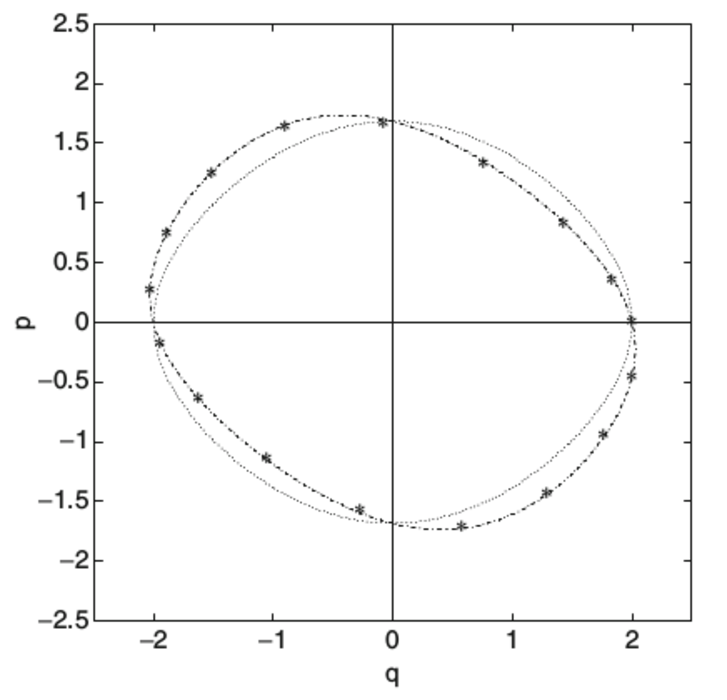
\includegraphics[width=.40\textwidth]{MetSinplektikoa}
%\caption{ \small Penduluaren problema: zenbakizko soluzioa (izarrak), benetako soluzioa (puntu lerroak) and perturbatutako soluzioa (marra lerroak) \cite{SSerna2015b}}
%\label{fig:MetSinplektikoa}
%\end{figure}

%Kasu orokorra, posible da $S_p$ Hamiltondar sistema perturbatua eraikitzea, zeinekin Euler sinplektikoa $p$ ordenakoa den. Beraz, konklusio gisa esango dugu, Hamiltondar sistema bati aplikatzen diogun metodo sinplektikoaren zenbakizko soluzioa, perturbatutako Hamiltondar sistema baten soluzio ia zehatza kontsideratu behar dugula. 

Metodo sinplektikoen propietate nagusienak azpimarratuko ditugu \cite{Hairer2006,JMSanz-Serna1994}.
\begin{enumerate}

\item Metodo sinplektikoek, energia oso ondo kontserbatzen dute.

Sistema Hamiltondarren $H(q,p)$ funtzio leunari sistemaren energia deitzen zaio. Soluzio zehatzak energia konstantea mantentzen du,
\begin{equation*}
H(p(t),q(t))=K, \ \ K \in \mathbb{R}.
\end{equation*}
Zenbakizko soluzioak ordea, ez du $H(p_n,q_n)$  konstante mantentzen. Integrazio metodoa sinplektikoa bada, aritmetika zehatzarekin energia errorea bornatua mantentzen da eta drift-ik edo handitzen doan desbideratzerik gabe. Koma-higikorreko aritmetikarekin, biribiltze errorearen eraginez energia errorea denboraren erro karratuaren arabera haziko da,
\begin{equation*}
\frac{H(p_n,q_n)-H(p_0,q_0)}{H(p_0,q_0)}=K \ \sqrt{t_n}.
\end{equation*}
non $K\in \mathbb{R}$ den.

\item Errorearen hedapen lineala.

Gehienetan, egoera aldagaien errorea $\mathcal{O}(h^p)$ da eta hazkundea lineala. Oro har, integratzaile arruntek errore hazkunde koadratikoa dute eta ondorioz, integrazio luzeetan portaera txarra azaltzen dute. Horregatik, metodo sinplektikoak egokiak dira integrazio luzetarako.

\item Metodo sinplektiko garrantzitsuenak simetrikoak dira.

\item
% Zuzenketa Joseba 04-05-2017
% Urrats luzera finkoa erabili behar da izaera sinplektikoa ez galtzeko \cite{JMSanz-Serna1994}.  Metodo gehienak eraginkorrak izateko, errore estimazio baten arabera integrazioan zehar urrats luzera egokitzen dute. Soluzioaren aldaketa azkarrak gertatzen diren uneetarako urratsa txikia, eta aldiz, urratsa handia soluzioa leuna den uneetarako.   

Izaera sinplektikoa mantendu beharrik ez dagoenean erabiltzen diren metodoek, eraginkortasuna hobetzeko, urrats luzera egokitu egiten dute, baina metodo sinplektikoak urrats luzera finkoarekin erabiltzen dira \cite{JMSanz-Serna1994}.

\end{enumerate} 

\section{Runge-Kutta metodo sinplektikoak}


1988. urtean, Sanz-Serna \cite{JMSanz-Serna1994} \emph{Gauss metodoa} sinplektikoa zela ohartu zen. Runge-Kutta metodo inplizitua da eta s-atalekin lor daitekeen ordena altuena du, alegia $p=2s$ ordenakoa da.  

\subsection{Runge-Kutta metodoak}

Runge-Kutta metodoak \cite{Hairer2006}, urrats bakarreko ekuazio diferentzial arrunten zenbakizko integrazio metodoak dira.  $b_{i}$, $a_{ij}$ eta $c_i=\sum\limits_{j=1}^{s} a_{ij} \ (1 \leq i,j \leq s)$ koefiziente errealek s-ataleko Runge-Kutta metodoa definitzen dute eta \emph{Butcher} izeneko taula moduan laburtu ohi dira, 
\begin{equation}
\label{eq:btchtaula}
\begin{array}{c|c}
  c & A  \\
  \hline
   &  b^T\\
\end{array}, \ \ \ \ \ \ \ \ \ \ \ \
\begin{array}{c|cccc}
  \ c_1 &  a_{11} & a_{12} & \dots & a_{1s}\\
  \ c_2 &  a_{21} & a_{22} & \dots &a_{2s}\\
  \ \vdots & \vdots & \vdots & \ddots & \vdots \\
  \ c_s & a_{s1} & a_{s2} & \dots & a_{ss}\\
  \hline
  \  & b_{1} & b_{2} & \dots & b_{s}\\
\end{array}
\end{equation}

(\ref{eq:ivp}) hasierako baliodun problemaren   $y_n \approx y(t_n)$ soluzioaren hurbilpena era honetan kalkulatzen da,
\begin{equation}  
y_{n+1}=y_n+h\sum^s_{i=1}{b_i \ f(t_n+c_ih,Y_{n,i})\ \ },\
\end{equation} 
%
non $Y_{n,i}$ atalak era honetan definitzen diren,
\begin{equation}
Y_{n,i}=y_n+\ h\ \sum^s_{j=1}{a_{ij}\ f(t_n+c_jh,Y_{n,j})}\ \ \ \ \ i=1 ,\dots, s.\
\end{equation} 

Runge-Kutta metodoak honako integrala hurbiltzen du:
\begin{equation*}
y(t_0+h)=y(t_0)+h \int_{0}^{1} \dot{y}(t_0+\theta h) d\theta,
\end{equation*} 
 hurrengo koadratura formularen bidez:
\begin{equation*}
 y_{1}=y_0+h\sum^s_{i=1}{b_i \ f(t_0+c_ih,Y_{i})}.
\end{equation*}
non $\dot{y}(t)=f(t,y(t))$ den, $b_i$ pisuak eta $c_i$ nodoak diren.

Era berean, $Y_{i} \approx y(t_0+c_ih)$ atal bakoitza ere, $0$ eta $c_i$ arteko integralaren hurbilketa da. Eta hauek ere, honako koadratura formularekin hurbiltzen dira:
\begin{equation*}
Y_{n,i}=y_0+h \sum_{j=1}^{s} a_{ij} \ f(t_0+c_jh,Y_{j}).
\end{equation*}

\subsubsection*{Metodo esplizituak (ERK) eta inplizituak (IRK)}
Runge-Kutta metodoak bi talde nagusitan bereiz ditzakegu: esplizituak (\emph {ERK}) non $\forall i\ge j, \ a_{ij}=0 $ eta inplizituak (\emph {IRK}) non $\exists i \ge j \ , a_{ij} \ne 0$ . 


\begin{enumerate}
\item \emph{ERK} metodoaren adibidea.

$s=4$ ataletako ERK metodo klasikoa era honetan definitzen da, 
\begin{equation*}
\begin{array}{c|cccc}
  \ 0   &    &    &     &      \\
  \ 1/2 & 1/2 &   &     &      \\
  \ 1/2 & 0   & 1/2  &  &      \\
  \ 1   & 0   & 0    &  1   &   \\
  \hline
  \     & 1/6 & 2/6  &  2/6 & 1/6 \\
  \end{array} \\
\end{equation*}

$Y_{n,i}$ atalak, esplizituki kalkula daitezke,
\begin{equation*}
Y_{n,i}=y_n+\ h\ \sum^{i-1}_{j=1}{a_{ij}\ f(t_n+c_jh,Y_{n,j})}\ \ \ \ \ i=1 ,\dots, s.
\end{equation*}  

\item \emph{IRK} metodoaren adibidea.

Honakoa da, $s=1$ ataleko \emph{puntu-erdiko metodo inplizituaren} (\emph{Implicit Midpoint method}) definizioa, 
\begin{equation*}
\begin{array}{c|c}
  \ 1/2 &  1/2\\
  \hline
  \     & 1 \\
\end{array} \\
\end{equation*}

$Y_{n,1}$ atala inplizituki definituta dago, eta honako ekuazio ez-lineala ebatzi behar da,
\begin{equation*}
Y_{n,1}=y_n+\ \frac{h}{2} \ f(t_n+\frac{h}{2},Y_{n,1}).
\end{equation*} 

\end{enumerate}

Lau-ataletako \emph{ERK}  metodo klasikoa, $p=4$ ordenakoa dugu. Ordena altuko \emph{ERK} metodoak aurkitzea konplexua da,  koefizienteek bete behar dituzten ordena baldintzen kopurua esponentzialki hazten baita. Esate baterako, ordena altuko \emph {ERK} metodo hauek aurkitu dira:  $s=11$ ataletako $p=8$ ordenako metodoa,  $s=17$ ataletako $p=10$ ordenako metodoa eta  $s=25$ ataletako $p=12$ ordenako metodoa.

Ordena altuko \emph{IRK} metodoak, \emph{ERK} metodoak baino modu errazagoan eraiki daitezke. \emph{Butcher-en sinplifikazio baldintzen}  \cite{Butcher2008} arabera definitzen dira.

% 04-05-2017 Josebaren zuzenketa 
%Ordena altuko \emph{IRK} metodoak, \emph{ERK} metodoak baino modu errazagoan eraiki daitezke.  \emph{Butcher sinplifikazio baldintza} hauen %\cite{Butcher2008} arabera definitzen dira,
%\begin{align}
%B(p) &: \ \ \ \sum\limits_{i=1}^{s} b_ic_i^{q-1} =\frac{1}{q}, \ \ & q=1,\dots,p. \\
%C(\eta) &: \ \ \ \sum\limits_{j=1}^{s} a_{ij}c_j^{q-1}  =\frac{c_i^q}{q},& \ \ i=1,\dots,s, \ q=1,\dots,\eta.\\
%D(\zeta) &:  \ \ \ \sum\limits_{i=1}^{s}  b_i c_i^{q-1}  a_{ij} = \frac{b_j}{q} (1-c_j^q),&  \ j=1,\dots,s, \  q=1,\dots,\zeta.
%\end{align}

%\ref{tab:irk} taulan, \emph{IRK} metodo nagusienak laburtu ditugu. 
%\begin{table}[h]
%\centering
%\caption{Runge-Kutta metodo inplizituak.}
%\label{tab:irk}       % Give a unique label
%\begin{tabular}{ l l l l c } 
% \hline
% \\
% Metodoa          &  Baldintzak             &                        &                 & Ordena \\
% \\
% \hline
% Gauss            &  $B(2s)$                & $C(s)$                 & $D(s)$          & $2s$    \\
% \hline
% Radau IA         &  $B(2s-1)$              & $C(s-1)$               & $D(s)$          & $2s-1$  \\
% \hline 
% Radau IIA        &  $B(2s-1)$             & $C(s)$                  & $D(s-1)$        & $2s-1$  \\
% \hline 
% Lobatto IIIA     &  $B(2s-2)$              & $C(s)$                 & $D(s-2)$        & $2s-2$  \\
% \hline
% Lobatto IIIB     &  $B(2s-2)$              & $C(s-2)$               & $D(s)$          & $2s-2$  \\
% \hline 
% Lobatto IIIC     &  $B(2s-2)$              & $C(s-1)$               & $D(s-1)$        & $2s-2$  \\
%  \hline
% \end{tabular}
%\end{table}

\subsubsection*{Sinplektikotasuna}

Sanz-Sernak  \cite{JMSanz-Serna1994} frogatu zuen,  Runge-Kutta metodoa sinplektikoa izan dadin honako baldintza betetzea nahikoa dela, baina aldi berean beharrezkoa dela:
\begin{equation}
\label{eq:simplektik}
b_{i}a_{ij}+b_{j}a_{ji}-b_{i}b_{j}=0, \ \ 1 \leqslant i,j \leqslant s.
\end{equation}

Baldintza honen arabera, Runge-Kutta metodo esplizituak, sinplektikoak ezin daitezkeela izan ondorioztatu daiteke. Bestalde, 1988. urtean, Sanz-Serna \cite{JMSanz-Serna1994} ohartu zen \emph{Gauss metodoa} sinplektikoa zela. 

\subsection{Gauss metodoa}

Gauss metodoak, bi ezaugarri nagusi dauzka: Runge-Kutta metodo sinplektikoa da eta bestetik, $s$-atalekin eduki daitekeen ordena altuena  dauka: $p=2s$. 

Kolokazio metodoak, zenbakizko integrazio metodo garrantzitsuak dira. Gauss metodoa, kolokazio metodoa da eta jarraian, ikuspegi honetatik definituko dugu. 

\subsubsection*{Kolokazio metodoak}

$c_1,c_2,\dots,c_s \ \ (0\leq c_i \leq 1)$ nodoetan oinarritutako kolokazio metodoak, $s$-mailako $u(t)$  \emph{polinomioa} definitzen du. Polinomioak honakoa betetzen du,
\begin{align*}
&u(t_0) =y_0, \\
&\dot{u}(t_0+c_ih) =f(t_0+c_i h, u(t_0+c_i h)), \ \ i=1,\dots,s.
\end{align*}
eta soluzioa 
\begin{equation*}
y_1=u(t_0+h)\approx y(t_0+h).
\end{equation*} 

Kolokazio metodoen zenbakizko soluzioak, diskretizazio puntuetan ez ezik, interpolazio polinomio batek modu jarraian emandako soluzioa adierazten du. 

Kolokazio metodoaren definizioa eta modu honetan kalkulatutako s-ataleko Runge-Kutta metodoa baliokideak dira \cite{Hairer2006}, 
\begin{equation}
a_{ij}=\int_{0}^{c_i} l_j(\tau) \ d\tau, \ \ b_i=\int_{0}^{1} l_i(\tau) \ d\tau
\end{equation}
%
non $l_i(\tau)$, Lagrangiar polinomioa dugun,
\begin{equation}
l_i(\tau)=\prod_{l\neq i} \frac{(\tau-c_l)}{(c_i-c_l)}.
\end{equation}
 
Aukeratutako $c_i$ ($1 \leq i \leq s)$ koefizienteen arabera, kolokazio metodo ezberdinak eraikitzen dira. Koefizienteak era honetan finkatzen badira,
\begin{equation*}
c_i=\frac{1}{2}(1+\bar{c}_i)
\end{equation*}
non $\bar{c}_i$, $s$-mailako Legendre polinomioaren zeroak diren, orduan Gauss kolokazio metodoa lortzen dugu.
Nodo hauetan oinarritutako Runge-Kutta metodoak, $p=2s$ ordena du.

\subsubsection*{Gauss metodoaren koefizienteak}

$s=1$, $s=2$ eta $s=3$ ataletako, Gauss kolokazio metodoaren \cite{Hairer2006} \emph{Butcher} koefiziente taulak \cite{Hairer2006} zehaztuko ditugu,
\begin{equation*}
\begin{array}{c|c}
  \frac{1}{2} & \ \frac{1}{2} \\
  \\
  \hline
   & 1 \\
\end{array} \ \ \ ,  \ \ \ \ \ \ \ \ \
\begin{array}{c|c c}
  \frac{1}{2}-\frac{\sqrt{3}}{6} & \ \frac{1}{4} & \ \frac{1}{4}-\frac{\sqrt{3}}{6} \\
  \\
  \frac{1}{2}+\frac{\sqrt{3}}{6} & \ \frac{1}{4}+\frac{\sqrt{3}}{6} & \ \frac{1}{4} \\
  \\
  \hline
         &  \frac{1}{2} & \ \frac{1}{2} \\
\end{array},
\end{equation*}

\begin{equation*}
\begin{array}{c|c c c}
  \frac{1}{2}-\frac{\sqrt{15}}{10} & \ \frac{5}{36} & \ \frac{2}{9}-\frac{\sqrt{15}}{15} & \ \frac{5}{36}-\frac{\sqrt{15}}{30} \\
  \\
  \frac{1}{2}   & \ \frac{5}{36}+\frac{\sqrt{15}}{24} & \ \frac{2}{9} & \ \frac{5}{36}-\frac{\sqrt{15}}{24} \\
  \\
  \frac{1}{2}+\frac{\sqrt{15}}{10}   & \ \frac{5}{36}+\frac{\sqrt{15}}{30} & \ \frac{2}{9}+\frac{\sqrt{15}}{15} & \ \frac{5}{36} \\
  \\
  \hline
  & \frac{5}{18} & \ \frac{4}{9} & \ \frac{5}{18}
\end{array}.
\end{equation*}

\subsubsection*{Gauss metodoaren propietateak}

Gauss metodoen ezaugarri nagusien artean honakoak daude:  
\begin{enumerate}
\item Metodo sinplektikoa da. Beraz, (\ref{eq:simplektik}) ekuazioak betetzen ditu. 
 
\item{Metodo simetrikoa da.}

Runge-Kutta metodoa simetrikoa izateko baldintzak hauek dira,
\begin{align*}
\label {eq:2}
 b_{i} &= b_{\sigma(i)} ,\ \  c_{\sigma(i)}= 1-c_{i}, \\
 b_{j} &= a_{\sigma(i),\sigma(j)}+a_{i,j}, \ \  i=1,2,\dots \lfloor s/2\rfloor
 \end{align*} 
non $\sigma(i)=s+1-i$.

Kolokazio metodo simetrikoetan, $c_i$ balioak integrazio urratsaren erdigunearekiko simetrikoak dira (ikus \ref{fig:simetrikoa} irudia  ).  
 \begin{figure}[h]
 \centering
 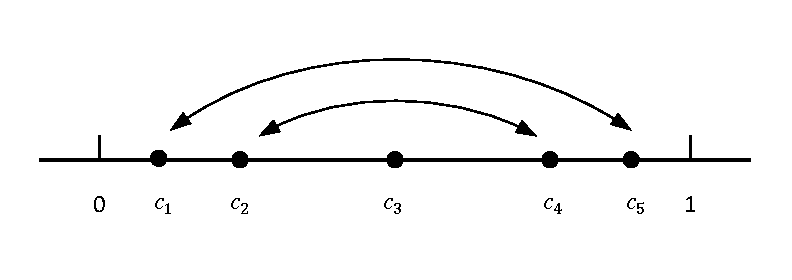
\includegraphics[width=.60\textwidth]{Simetria}
 \caption[Kolokazio metodoen simetria]{ \small Kolokazio metodoen simetria}
 \label{fig:simetrikoa}
 \end{figure}
 
\item{Ordena altuko metodoa.}
Edozein ordenako Gauss metodoa eraiki daiteke. Doitasun handiko konputazioetarako ordena altuko metodoak beharrezkoak dira: doitasun bikoitzeko aritmetikan (biribiltze unitatea $u\approx10^{-16}$) ~$p\geqslant8$ ordenako metodoak gomendagarriak dira eta doitasun laukoitzeko aritmetikan (biribiltze unitatea $u\approx10^{-35}$) ordena altuagoko metodoak beharrezkoak dira.  

\item{Metodo orokorra da.}
Gauss metodoa edozein ekuazio diferentzial ebazteko erabil daiteke. Sistema Hamiltondarren kasuan, ez du zertan banagarria izan  Hamiltondarrak.

\item{Paralelizagarria da.}
Ekuazio diferentzial garestiak ditugunean, $s$-ataletako funtzioen konputazioak ($f(Y_i), \ i=1,\dots,s$) paraleloan kalkula daitezke.  

\item{Kolokazio metodoa da.}
Zenbakizko soluzioak diskretizazio puntuetan ez ezik, urrats bakoitzaren integrazio tarte osoaren polinomio interpolatzaile batek modu jarraian emandako soluzioa adierazten du.

%\item{A-stability and B-stability.}
%A-stable methods have a central role in the numerical solution of stiff problems and Gauss methods are likely candidates.

\item{Birparametrizazioa.}
Metodo sinplektiko inplizituetan, birparametrizazio teknika zuzenean aplika daiteke. Eguzki-sistemaren integrazioetarako tresna baliagarria dela frogatu da \cite{Fukushima2007}. 
  
\end{enumerate}

      
\subsection{IRK inplementazioa}

\subsubsection*{IRK algoritmoa}

\emph{IRK} metodoaren inplementazio orokorra, \ref{alg:IRK1} algoritmoan ikus daiteke. Inplementazio eraginkorra egin ahal izateko, algoritmo horretako bete behar garrantzitsuenak ondo kudeatzea komeni da.

\begin{algorithm}[H]
 \BlankLine
  $y_0=y(t_0)$\;
 \BlankLine
  \For{$n\leftarrow 0$ \KwTo ($endstep-1$)}
  {
   \BlankLine
   $k=0$\;
   \text{Hasieratu}  $Y_{n,i}^{[0]} \ \ , \ \ i=1,\dots,s $\;
    \BlankLine
   \While{ (konbergentzia lortu)}
   {
    \BlankLine
    $k=k+1$\; 
    $F_{n,i}^{[k]}=f(t_n+c_ih,Y_{n,i}^{[k-1]}) $\;
    \text{Askatu} ($Y_{n,i}^{[k]}=y_{n}+ h \ \sum\limits_{j=1}^{s} a_{ij} F_{n,j}^{[k]}$) \; 
    $\text{konbergentzia} \leftarrow \text{GeratzeErizpidea}(Y^{[k]},Y^{[k-1]}) $\; 
   }
   \BlankLine
    $\delta_n=h \ \sum\limits_{i=1}^{s} b_i F_{n,i}$\;
    $y_{n+1}=y_{n}+ \delta_n $\;
   \BlankLine
 }
 \caption{IRK Algoritmo orokorra}
 \label{alg:IRK1}
\end{algorithm}


\subsubsection*{Atalen hasieraketa}
\label{ss:2.2.3.2}

Atalen hasieraketa egokia definitu behar da. Aukera sinpleena $Y_{n,i}^{[0]}=y_{n}$ hasieratzea da, baina aurreko urratseko atalen informazioa erabiliz hurbilketa hobea lor daiteke \cite{Hairer2006}. Aurreko urratseko atalak interpolatzen dituen polinomioaren 
bidezko hasieraketa era honetan adieraz dezakegu,
\begin{equation*}
Y_{n,i}^{[0]}=g(Y_{n-1,i}) \ , \ i=1, \dots, s. 
\end{equation*}

Aurreko urratseko $Y_{n-1,i}$~atalak eta $(t_{n-1}+h,y_{n})$ zenbakizko soluzioa ezagututa, polinomio interpolatzailearen bidez, urrats berriaren atalen hasieraketa  $Y_{n,i}^{[0]}$ kalkula daiteke (\ref{fig:AtalHasieraketa} Irudia). 
\begin{figure}[h!]
\centerline{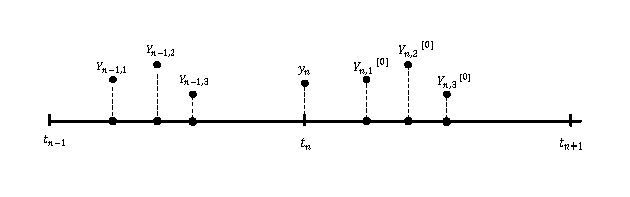
\includegraphics[width=14cm, height=4cm] {YiAtalenHasieraketa}}
\caption[Atalen hasieraketa: interpolazioa]{Atalen hasieraketa: interpolazioa}
\label{fig:AtalHasieraketa}
\end{figure}

\begin{enumerate}
\item ($n-1$). urratsaren informazioa.
\begin{align*}
\left \{ \begin{array}{c}
Y_{n-1,i} =y_{n-1}+h \sum\limits_{j=1}^{s} a_{ij} f(Y_{n-1,j}),\\
y_n =y_{n-1}+h \sum\limits_{j=1}^{s} b_j f(Y_{n-1,j}),\\
\end{array} \right.\\
\ \Rightarrow \ \ 
Y_{n-1,i}&=y_n+h \sum\limits_{j=1}^{s} (a_{ij}-b_j) f(Y_{n-1,j}).
\end{align*}

\item Polinomio interpolatzailea.
\begin{equation*}
P(t)=  l_1(t) Y_{n-1,1}+\dots+l_s(t) Y_{n-1,s}+l_{s+1}(t) y_n
\end{equation*}
  
non $l_i(t)$ Lagrangiar polinomioa dugun,
\begin{equation*}
 l_i(t)=\prod_{l\neq i,l=1}^{s+1} \frac{(t-(t_{n-1}+hc_l))}{(c_i-c_l)}, \ \ c_{s+1}=1.
\end{equation*}

\item Atalen hasieraketa.
\begin{equation*}
Y_{n,i} \approx Y_{n,i}^{[0]}= P(t_n+hc_i) = y_n+ h \sum\limits_{j=1}^{s} \lambda_{ij}f(Y_{n-1,j}).
\end{equation*}

\end{enumerate}

Modu honetan s-ataletako IRK metodo bakoitzari dagokion, $\lambda_{ij}$ interpolaziorako koefizienteak lor daitezke. Polinomio interpolatzailearen bidezko hasieraketa, emandako urratsa oso handia ez bada eta problema zurruna ez bada, ona izango da. Era berean aipatu nahi genuke, atal askotako metodoetan (adibidez $s=16$)  interpolaziozko koefizienteen kalkuluan ezabapen arazoak doitasun handian lan egitera behartzen gaituela interpolaziozko hasieraketa ona izateko.   

Laburta-ren lanean \cite{Laburta1998}, hasieraketa aurreratuei buruzko informazioa aurki daiteke.  


\subsubsection*{Iterazio metodoa}

\emph{IRK} metodoen erronka handiena, ekuazio-sistema ez-linealaren zenbakizko soluzioaren inplementazio eraginkorra da \cite{Hairer2006,SSerna2015b}. Problema ez-zurrunetarako, atalen hasieraketa ($Y_i^{[0]}$) egoki bat duen puntu-finkoaren iterazioa erabil daiteke. Problema zurrunetarako, puntu-finkoaren iterazioan konbergentzia egon dadin, urrats tamaina txikiegia erabiltzea behartuko luke eta ondorioz, Newtonen iterazio sinplifikatua erabili ohi da.  

\begin{enumerate}

\item Puntu-finkoaren iterazioa

\begin{algorithm}[H]
  \For{ (k=1,2,\dots)}
  {
   $F_{i}^{[k]}=f(t_n+c_ih,Y_i^{[k-1]})$\;
   $Y_{i}^{[k]}=y_{n}+ h \ \sum\limits_{j=1}^{s} a_{ij} F_{j}^{[k]} , \ \  i=1,\dots,s$\; 
  }
 \caption{Puntu-finkoaren iterazioa}
 \label{alg:rkpf}
\end{algorithm}

Konbergentzia $\|Y^k-Y\|=\mathcal{O}(h) \|Y^{k-1}-Y\|$.


\item Newtonen iterazioa 

Newtonen iterazio bakoitza konputazionalki garestia da. Batetik,  $\frac{\partial f}{\partial y}(t_n+c_ih,Y_i^{[k-1]}), \ i=1,\dots,s$ Jacobiarrak ebaluatu behar dira. Bestetik, s-ataletako IRK metodoa eta  d-dimentsioko ekuazio diferentzialen sistema baditugu, $sd \times sd$ dimentsioko sistema lineala ebatzi behar da.    

\begin{algorithm}[H]
  \For{ (k=1,2,\dots)}
  {
   $r_{i}^{[k]}=-Y_i^{[k-1]}+y_n+h \ \sum\limits_{j=1}^{s} a_{ij} f(t_n+c_ih,Y_j^{[k-1]}) $\;
   Askatu $\triangle Y_i^{[k]}$\;
   $\triangle Y_i^{[k]}-h \ \sum\limits_{j=1}^{s} a_{ij} \frac{\partial f}{\partial y}(t_n+c_jh,Y_j^{[k-1]}) \ \triangle Y_j^{[k]}=r_i^{[k]}$\;
   $Y_i^{[k]}=Y_i^{[k-1]}+\triangle Y_i^{[k]}, \ \  i=1,\dots,s$\; 
  }
 \caption{Newton metodoaren iterazioa}
\end{algorithm}

Konbergentzia $\|Y^k-Y\|=\mathcal{O}(h^2) \|Y^{k-1}-Y\|$.

\end{enumerate}

\subsubsection*{Hamiltondar banagarriak (Metodo partizionatuak)}

Era honetako ekuazio diferentzialak, garrantzitsuak dira,
\begin{equation*}
\dot{p}=f(q), \ \ \dot{q}=g(p).
\end{equation*}

Esaterako, Hamiltondar banagarriak $H(q,p)=T(p)+U(q)$ eta bigarren ordenako ekuazio diferentzialak $\ddot{q}=f(q)$ era honetako ekuazio diferentzialen kasu partikularrak dira.

Zenbakizko soluzioa $(p_{n+1},q_{n+1}) \approx (p(t_{n+1}),q(t_{n+1}))$ era honetan kalkula daiteke \cite{JMSanz-Serna1994},
\begin{align}
\begin{split}
&p_{n+1}=p_n+ h \sum\limits_{i=1}^{s} b_i \ f(t_n+c_ih,Q_{n,i}),\\
&q_{n+1}=q_n+ h \sum\limits_{i=1}^{s} b_i \ g(t_n+c_ih,P_{n,i}),
\end{split}
\end{align}

non $P_{n,i},Q_{n,i} \ i=1,\dots,s$ atalak, honako ekuazio-sistemaren bidez definitutakoak diren, 
\begin{align}
\begin{split}
&P_{n,i} =p_n+ h \sum\limits_{j=1}^{s} a_{ij} \ f(t_n+c_jh,Q_{n,j}), \\
&Q_{n,i} =q_n+ h \sum\limits_{j=1}^{s} a_{ij} \ g(t_n+c_jh,P_{n,j}).
\end{split}
\end{align}

Problema hauetan,  funtsean puntu-finkoaren iterazioa (\ref{alg:rkpf}~algoritmoa) aplikatzean, Hamiltondarraren egiturari esker, iterazioaren konbergentzia hobetu egiten da,   

\begin{algorithm}[H]
  \For{ (k=1,2,\dots)}
  {
  \BlankLine
   $P_{n,i}^{[k]}=p_{n}+ h \ \sum\limits_{j=1}^{s} a_{ij} \ f(t_n+c_jh,Q_{n,j}^{[k-1]})$\; 
   $Q_{n,i}^{[k]}=q_{n}+ h \ \sum\limits_{j=1}^{s} a_{ij} \ g(t_n+c_jh,P_{n,j}^{[k]}), \ \ \ \ i=1,\dots,s $\; 
  }
 \caption{Puntu-finkoaren iterazioa (Metodo partizionatuak)}
 \label{alg:rkfppart}
\end{algorithm}


\subsubsection*{Bigarren ordenako EDA}

Bigarren ordenako ekuazio diferentzialen $\ddot{q}=f(q)$ azterketa egiteko, lehen ordenako ekuazio diferentzial moduan idatziko dugu,
\begin{equation*}
\dot{p}=f(q), \ \ \dot{q}=p.
\end{equation*}

Zenbakizko soluzioa $(p_{n+1},q_{n+1}) \approx (p(t_{n+1}),q(t_{n+1}))$ era honetan kalkula daiteke \cite{JMSanz-Serna1994},
\begin{align}
\begin{split}
&p_{n+1}=p_n+ h \sum\limits_{i=1}^{s} b_i \ f(t_n+c_ih,Q_{n,i}),\\
&q_{n+1}=q_n+ h p_{n} + h^2 \sum\limits_{i=1}^{s} \beta_i \ f(t_n+c_ih,Q_{n,i}),
\end{split}
\end{align}
%
non $Q_{n,i}, \ i=1,\dots,s$ atalak, honako ekuazio-sistemen bidez definitutakoak diren, 
\begin{align}
Q_{n,i}=q_n+ h\gamma_i p_n+ h^2 \sum\limits_{j=1}^{s} \tilde{a}_{ij} \ f(t_n+c_jh,Q_{n,j}).
\end{align}

Bigarren ordenako ekuazio diferentzialen kasuan, puntu-finkoaren iterazioa modu eraginkorrean aplika daiteke,

\begin{algorithm}[H]
  \For{ (k=1,2,\dots)}
  {
   $Q_{n,i}^{[k]}=q_{n}+h \gamma_i p_{n}+ h^2 \ \sum\limits_{j=1}^{s} \tilde{a}_{ij} f(t_n+c_jh,Q_{n,j}^{[k-1]}) $\;  
  }
 \caption{Puntu-finkoaren iterazioa (bigarren ordenako EDA)}
\end{algorithm} 

% 04-05-2017 Joseba zuzenketa.
%IRK algoritmoa-III (bigarren ordenako EDA).
%
%\begin{algorithm}[H]
% \BlankLine
%  \For{$n\leftarrow 0$ \KwTo ($endstep-1$)}
%  {
%   \BlankLine
%   Hasieratu  $Q_{n,i}^{[0]} \ \ , \ \ i=1,\dots,s $\;
%    \BlankLine
%   \While{ (konbergentzia lortu)}
%   {
%    \BlankLine 
%    $F_{n,i}=f(t_n+c_ih,Q_{n,i}) \ \ , \ \  i=1,\dots,s$\;
%    $Q_{n,i}=q_n+ h\gamma_i p_n+ h^2 \sum\limits_{j=1}^{s} \tilde{a}_{ij} \ f(t_n+c_jh,Q_{n,j}) \ \ , \ \  i=1,\dots,s$\;  
%   }
%   \BlankLine
%    $\delta p_n=h \ \sum\limits_{i=1}^{s} b_i F_{n,i}$\;
%    $\delta q_n=h^2 \sum\limits_{i=1}^{s} \beta_i F_{n,i}$\;    
%    $p_{n+1}=p_{n}+ \delta p_n $\;
%    $q_{n+1}=q_{n}+ h\gamma_i p_n+\delta q_n $\;
%   \BlankLine
% }
% \caption{IRK algoritmoa-III (bigarren ordenako EDA)}\label{alg:IRK2}
%\end{algorithm}


\subsubsection*{Batura Konpensatua}

Zenbakizko integrazioaren urrats bakoitzean,
\begin{equation*}
y_{n+1}=y_{n}+ \delta_n,
\end{equation*}
batura kalkulatu behar dugu. Normalean $|\delta_n| \ll |y_n| $ izango da eta integrazio luzeetan, batura honek soluzioaren doitasun galera eragingo du. Hau ekiditeko \emph{batura konpentsatua} izeneko  teknika \cite{Muller2009,Higham2002,Hairer2006} erabili ohi da. Teknika hau 4.atalean deskribatu dugu eta zehaztapenak \ref{alg:batkp} algoritmoan eman ditugu.
 

\section{Konposizio eta splitting metodoak}
\label{s:KonSpl}

Konposizio eta splitting ideietan oinarrituz, aplikazio eremu ezberdinetarako hainbat integratzaile sinplektiko \cite{SSerna2015b} garatu dira. Metodo hauek ez dira orokorrak, problema zehatzetan aplikagarriak baizik, eta metodo oso eraginkorrak dira.

\subsection{Konposizio metodoak}
\label{ss:Konp}

Konposizio metodoak, oinarrizko metodo bat edo gehiago konposatuz eraikitako zenbakizko integrazio metodoak dira \cite{Hairer2006}.  Oinarrizko metodoekin segidan exekutatutako azpi-urrats kopuru batek, konposizio metodoaren integrazioaren urrats bat osatzen du. Helburua, orden baxuko metodo batetik abiatuta, ordena altuko metodoa eraikitzea da; konposizio metodoak, konposatutako oinarrizko metodoaren propietateak (simetrikoa, sinplektikoa,\dots) jasotzen ditu. 

\subsubsection*{Konposizio orokorrak}
$\phi_h$ oinarrizko metodoa eta $\gamma_1,\dots,\gamma_s$ zenbaki errealak emanik, urrats luzera hauen $\gamma_1 h,\gamma_2 h,\dots,\gamma_s h$ konposaketari dagokion konposizio metodoa era honetan definituko dugu,
\begin{equation}
\Psi_h=\phi_{\gamma_s h} \circ \dots \circ \phi_{\gamma_{1 h}}.
\end{equation}

\subsubsection*{Algoritmoa}
Jarraian, s-ataletako konposizio metodoen inplementazioaren algoritmo orokorra laburtu dugu.

\begin{algorithm}[H]
 \BlankLine
  \For{$n\leftarrow 0$ \KwTo $(endstep-1)$}
  {
   \BlankLine
    $Y_{0,n}=y_{n} $\;
    \BlankLine
   \For{$i=1,2,\dots,s$}
   {
    \BlankLine 
    $Y_{i,n}=\phi_{\gamma_i h}(Y_{i-1,n})$\;
   }
   \BlankLine
    $y_{n+1}=Y_{s,n}$\;
   \BlankLine
 }
 \caption{Konposizio metodoen inplementazioa}
 \label{alg:konp}
\end{algorithm}
 
Konposizio metodoen inplementazioaren ezaugarri nagusienak hauek dira:
\begin{enumerate}
\item{Esplizituak dira.}

Konposizio metodo hauek esplizituak dira. Metodo hauetan ez da ekuazio-sistemarik askatu behar, eta beraz inplementazioa sinplea da. 

\item{Sekuentzialak dira.}

Azpi-urrats bakoitzaren kalkulua modu sekuentzialean ($i=1,\dots,s$) egin behar dugu.

\item{Memoria gutxi behar dute.}

Ez da tarteko baliorik eta datu-egitura berezirik memorian gorde behar.   

\item{Bigarren ordenako ekuazio diferentzialentzat egokiak dira.}

Bigarren ordenako ekuazio diferentziala ($\ddot{q}=f(p)$), \emph{Störmer-Verlet} (\emph{Leapfrog} izenarekin ere ezaguna) metodoan oinarritutako, $s$-ataletako konposizio metodoarekin integratzeko, urrats bakoitzean ekuazio diferentzialaren $s$ balioztapen egin behar ditugu:
\begin{align}
\begin{split}
&q_{{n+1}/{2}}=q_n+\frac{h}{2} \ p_n,\\
&p_{n+1}=p_n+h \ f(q_{{n+1}/{2}}),\\
&q_{n+1}=q_{{n+1}/{2}}+\frac{h}{2} \ p_{n+1}.
\end{split}
\label{eq:stverlet}
\end{align}


\end{enumerate}

\subsubsection*{Konposizio simetrikoak}

$\phi_h$ oinarrizko metodoa $p=2$ ordenakoa eta simetrikoa izanik, era honetako konposizioak aurkitu dira,
\begin{equation}
\Psi_h=\phi_{\gamma_s h} \circ \phi_{\gamma_s-1 h} \circ \dots \circ \phi_{\gamma_{2 h}} \circ \phi_{\gamma_{1 h}} 
\end{equation}
non $\gamma_s=\gamma_1, \gamma_{s-1}=\gamma_2,\dots$ 

\subsubsection*{CO1035: $10$ ordenako konposizio metodoa}

Sofroniou eta Spaletta-ren \cite[~2004]{Sofroniou2005} $s=35$ eta $p=10$ ordenako metodoa, orain arteko  ordena altueneko konposizio metodo eraginkorrena bezala har daiteke (\ref{tab:co1035} taula). Konposizio metodo simetrikoa: oinarrizko metodoa simetrikoa eta $p=2$ ordenakoa  da.  

\begin{table}[h]
\caption[CO1035 konposizio metodoa] 
{\small{10 ordenako konposizio metodoa \cite[~158.or]{Hairer2006} (CO1035)}}
\label{tab:co1035}       % Give a unique label
\centering
\resizebox{\textwidth}{!}{%
\begin{tabular}{ c c c c } 
 \hline
 Koefizientea         &  Balioa  & Koefizientea & Balioa \\
 \hline
 $\gamma_1=\gamma_{35}$ & 0.07879572252168641926390768 &  $\gamma_{10}=\gamma_{26}$ & -0.39910563013603589787862981 \\
 $\gamma_2=\gamma_{34}$ & 0.31309610341510852776481247 & $\gamma_{11}=\gamma_{25}$ & 0.10308739852747107731580277 \\ 
 $\gamma_3=\gamma_{33}$ & 0.02791838323507806610952027 & $\gamma_{12}=\gamma_{24}$ & 0.41143087395589023782070412 \\
 $\gamma_4=\gamma_{32}$ &-0.22959284159390709415121340 & $\gamma_{13}=\gamma_{23}$ & -0.00486636058313526176219566 \\ 
 $\gamma_5=\gamma_{31}$ & 0.13096206107716486317465686 & $\gamma_{14}=\gamma_{22}$ & -0.39203335370863990644808194 \\  
 $\gamma_6=\gamma_{30}$ & -0.26973340565451071434460973 & $\gamma_{15}=\gamma_{21}$ & 0.05194250296244964703718290 \\  
 $\gamma_7=\gamma_{29}$ & 0.07497334315589143566613711 & $\gamma_{16}=\gamma_{20}$ & 0.05066509075992449633587434 \\ 
 $\gamma_8=\gamma_{28}$ & 0.11199342399981020488957508 & $\gamma_{17}=\gamma_{19}$ & 0.04967437063972987905456880 \\  
 $\gamma_9=\gamma_{27}$ & 0.36613344954622675119314812 &$\gamma_{18}$ & 0.04931773575959453791768001 \\ 
   \hline
 \end{tabular}}
\end{table}

Hamiltondarra $H=H_1+H_2$ izanik, eta \emph{Stömer-Verlet} metodoan (\ref{eq:stverlet}) ($\phi_h=\varphi_{h/2}^{H_1} \circ \varphi_{h}^{H_2} \circ \varphi_{h/2}^{H_1}$) oinarritutako konposizio metodoaren inplementazioaren zehaztasunak honakoak dira.
\begin{enumerate}
\item Konposizio metodo orokorra.
\begin{equation*}
\Psi_h =\phi_{\gamma_{s h}} \circ \phi_{\gamma_{s-1 h}} \circ \dots \circ \phi_{\gamma_{2 h}} \circ \phi_{\gamma_{1 h}}
\end{equation*}

\item \emph{Stömer-Verlet} oinarrizko metodoaren konposizio metodoa,
\begin{equation*}
\Psi_h =(\varphi_{h \gamma_s/2}^{H_1} \circ \varphi_{h \gamma_s}^{H_2} \circ \varphi_{h \gamma_s/2}^{H_1}) \circ \dots 
       \circ
       (\varphi_{h \gamma_1/2}^{H_1} \circ \varphi_{h \gamma_1}^{H_2} \circ \varphi_{h \gamma_1/2}^{H_1}).  
\end{equation*}

\item Jarraian dauden $\varphi^{H_1}$ fluxuak era honetan elkartu daitezke,
\begin{equation*}
\Psi_h=\varphi_{h a_{s+1}}^{H_1} \circ \varphi_{h b_s}^{H_2} \circ \varphi_{h a_s}^{H_1} \circ \cdots 
       \circ
       \varphi_{h b_2}^{H_2} 
       \circ
       \varphi_{h a_2}^{H_1} \circ \varphi_{h b_1}^{H_2} \circ \varphi_{h a_1}^{H_1}  
\end{equation*}
non $a_1=a_{s+1}=\gamma_1/2$, $b_i=\gamma_i$, $a_k=(\gamma_k+\gamma_{k-1})/2$, $i=1,\dots,s$ eta $k=2,\dots,s$.

\item Azkenik, integrazioaren tarteko urratsetan, lehen atala $\varphi_{h a_{s+1}}^{H_1}$ eta azkena $\varphi_{h a_1}^{H_1}$ bakar batean elkartu daitezke,
\begin{equation*}
\Psi_h=\varphi_{h 2 a_{s+1}}^{H_1} \circ \varphi_{h b_s}^{H_2} \circ \varphi_{h a_s}^{H_1} \circ \cdots 
\circ \varphi_{h b_2}^{H_2} 
\circ
\varphi_{h a_2}^{H_1} \circ \varphi_{h b_1}^{H_2}.
\end{equation*}

\end{enumerate}


\subsection{Splitting metodoak}
\label{ss:Splt}

\emph{Splitting metodoak}, $f: \mathbb{R}^d \rightarrow \mathbb{R}^d$ sistema osoa integratzeko, $f^{[i]}$ ($f=\sum\limits_{i=1}^{m} f^{[i]}$) azpiproblemetan deskonposatu daitezkeen ekuazio diferentzialetarako zenbakizko integrazio metodoak dira \cite{SSerna2015b,Hairer2006}.

Splitting metodoa modu errazean aplika daiteke, $H$ Hamiltondarra, $H=H_1+H_2$ eran bana daitekeenean eta Hamiltondar bakoitzari dagokion sistema modu esplizituan integratu daitekeenean.  

\subsubsection*{Splitting arruntak}

$H_1 \ \text{eta} \ H_2$ sistemen fluxu zehatzak $\varphi_t^{[H_2]}$ eta $\varphi_t^{[H_1]}$ izendatzen baditugu, honako splitting metodoak definituko ditugu:

\begin{enumerate}

\item Lie-Trotter splitting $1$ ordenako metodoak,
\begin{equation}
\phi_h = \varphi_h^{[H_2]} \circ \varphi_h^{[H_1]} \ \ \ edo \ \ \ \phi_h^{*} = \varphi_h^{[H_1]} \circ \varphi_h^{[H_2]}.
\label{eq:LieT}
\end{equation}


\paragraph*{Adibidea.}

Era honetako Hamiltondar banagarrietarako $H(q,p)=T(p)+V(q)$, $H_1=T$ eta $H_2=V$ izanik, zati bakoitzari dagokion fluxua era honetan definitzen da,
\begin{equation*}
\varphi_t^{[H_1]}=(p,q+t\triangledown T(p)), \ \ \varphi_t^{[H_2]}=(p-t\triangledown V(q),q). 
\end{equation*}
Adibide honen splitting metodo partikularra, \emph{Euler metodo sinplektiko} izenarekin ezaguna da,
\begin{align*}
p_{n+1}&=p_{n}-h \triangledown V(q_{n+1}), \\
q_{n+1}&=q_{n}+h \triangledown T(p_n).
\end{align*}  
   

\item Strang-Marchuk splitting $2$ ordenako metodo simetrikoa,
\begin{equation}
\phi_h =  \varphi_{{h}/{2}}^{[H_1]} \circ \varphi_h^{[H_2]} \circ \varphi_{{h}/{2}}^{[H_1]}.
\end{equation} 

\paragraph*{Adibidea.}

Hamiltondar banagarrietarako $H(q,p)=T(p)+V(q)$, ~\emph{Störmer-Verlet metodo} ezaguna lortzen da,
\begin{align*}
&q_{{n+1}/{2}} =q_n+\frac{h}{2} \triangledown T(p_n), \\
&p_{n+1} =p_n-h \triangledown V(q_{{n+1}/{2}}), \\
&q_{n+1} =q_{{n+1}/{2}}+\frac{h}{2} \triangledown T(p_{n+1}).
\end{align*}

\end{enumerate}

\subsubsection*{Fluxu zehatza eta zenbakizko fluxua konbinatuz}
Demagun, sistemaren bi fluxu zehatzetariko bat $\varphi_t^{[H_1]}$ edo $\varphi_t^{[H_2]}$ ezin daitekeela kalkulatu. Kasu honetan ere splitting teknika aplika daiteke  metodo sinplektikoak eraikitzeko . Adibidez, $\varphi_t^{[H_2]}$ ezezaguna bada eta Lie-Trotter teknika aplikatuz,

\begin{equation*}
\phi_h=\varphi_h^{[H_1]} \circ \phi_h^{[H_2]}, \ \ \ \ \ \  \phi_h^{*}=\phi_h^{[H_2]} \circ \varphi_h^{[H_1]},
\end{equation*}
%
eta lortzen den zenbakizko metodoak, $\phi_t^{[H_2]}$ zenbakizko metodoaren propietateak mantentzen ditu. 

\subsubsection*{Splitting orokorrak}

Aurreko splitting metodoen (\ref{eq:LieT}) orokorpena modu honetan zehaztuko dugu,
\begin{equation}
\phi_h = \varphi_{\beta_s h}^{[H_2]} \circ \varphi_{\alpha_s h}^{[H_1]} \circ \varphi_{\beta_s-1 h}^{[H_2]} 
\circ \cdots \circ \varphi_{\beta_1 h}^{[H_2]} \circ \varphi_{\alpha_1 h}^{[H_1]} .
\end{equation}
%
non $\beta_i$, $\alpha_i$ koefizienteak ($\sum \beta_i=1$, $\sum \alpha_i=1$) metodoaren ordena definitzen duten.


\subsubsection*{Algoritmoa}

\emph{Splitting metodoen} inplementazio orokorra \ref{alg:split} algoritmoan ikus daiteke:

\begin{algorithm}[H]
 \BlankLine
  \For{$n\leftarrow 0$ \KwTo ($endstep$-1)}
  {
   \BlankLine
    $Y_{0,n}=y_{n-1} $\;
    \BlankLine
   \For{i=1,2,...,s}
   {
    \BlankLine 
    $Y_{i,n}=(\varphi^{[H_2]}_{\beta_i h} \circ \varphi^{[H_1]}_{\alpha_i h})(Y_{i-1,n})$\ ;
   }
   \BlankLine
    $y_{n+1}=Y_{s,n}$\;
   \BlankLine
 }
 \caption{Splitting metodoak}
 \label{alg:split}
\end{algorithm}

Splitting metodoen inplementazioarentzat, konposizio metodoen algoritmoei buruz aipatutako ezaugarri berdinak errepikatu beharko genituzke (esplizituak dira, sekuentzialki exekutatzen dira, memoria gutxi, \dots). 

\subsection{Eguzki-sistemari egokitutako splitting metodoak}

Har dezagun, N-gorputzeko problema grabitazionalaren Hamiltondarra,
\begin{equation*}
H(q,p)=T(p)+U(q).
\end{equation*}

Eguzki-sistemaren integraziorako erabiltzen diren koordenatu sistema nagusiak, \emph{Jacobi} eta koordenatu heliozentrikoak dira \cite{Wisdom2006,Farres2013}.  Bi koordenatu sistema hauekin, Hamiltondarra beste modu honetan berridatz daiteke,
\begin{equation*}
H=H_A+\epsilon H_B,  \ \ \ \ |H_B|\ll|H_A|,
\end{equation*}
non alde nagusia $H_A$ planeta bakoitzaren eguzkiaren inguruko mugimendu Kepleriarra den eta $H_B$ aldiz, planeten arteko interakzioek eragiten duten perturbazio txikia. Jacobi koordenatuetan $H_B$-k ez dauka $p$-ren menpekotasunik, heliozentrikoetan, ordea, bi aldagaien menpekotasuna dauka (ikus \ref{erans:B2} eranskinean):
\begin{align*}
&H_{Jab}=H_A(p,q)+H_B(q), \\
&H_{Hel}=H_A(p,q)+H_B(p,q), 
\end{align*}       

$H_A(p,q)$ (mugimendu Kepleriarrari dagokion zatia), Kepler-en fluxua kalkulatzen duen inplementazio bat aplikatuz (\ref{ss:342}~atala) zehazki kalkulatuko da.

Eguzki-sistemaren problema grabitazionalari egokitutako zenbakizko bi integratzaile sinplektiko azalduko ditugu. Lehena, Laskar-ek eta Robutel-ek \cite{Laskar2001} definitutako \emph{$SABAC_4$} integratzailea eta bigarrena, Blanes et al. \cite{Blanes2013,Farres2013} definitutako \emph{$ABAH1064$} integratzailea. 


\subsubsection*{$SABAC_4$ integratzailea}

Laskarrek \cite[$2001$]{Laskar2001}, $CSABA_n$ eta $CSBAB_n$ integratzaile sinplektikoak proposatu zituen. Metodo hauek koefiziente positiboekin eraikitako metodo sinplektikoak dira eta $\mathcal{O}(h^{k} \epsilon+ h^{4} \epsilon^2)$ ordenakoak dira, $n$ bikoitia denean $k=n+2$ izanik eta $n$ bakoitia denean $k=n+3$ izanik. 

Eguzki-sistemaren epe luzeko integrazioan \cite{Laskar2011} erabilitako $CSABA_4$ integratzailea deskribatuko dugu. Hamiltondarra $H=H_A+\epsilon H_B$ bada, era honetan definituko dugu metodoa,
\begin{align*}
&SABA_4 =\varphi^{[A]}_{c_1 h} \circ \varphi^{[B]}_{d_1 h} \circ \varphi^{[A]}_{c_2 h} \circ \varphi^{[B]}_{d_2 h}
         \circ  \varphi^{[A]}_{c_3 h}   \circ
          \varphi^{[B]}_{d_2 h} \circ \varphi^{[A]}_{c_2 h} \circ   \varphi^{[B]}_{d_1 h}\circ  \varphi^{[A]}_{c_1 h}, \\
&CSABA_4 =\varphi^{[B]}_{-c/2} \circ SABA_4 \circ \varphi^{[B]}_{-c/2},          
\end{align*}
eta koefizienteak \ref{tab:CSABA4} taulan zehaztu ditugu.
 
\begin{table}[h!]
\centering
\caption[$CSABA_4$ splitting metodoa] 
{\small{$CSABA_4$ splitting metodoa \cite{Laskar2001}}}
\label{tab:CSABA4}       % Give a unique label
\begin{tabular}{ c c | c c} 
 \hline
 Koefiziente         &  Balioa  & Koefiziente         &  Balioa  \\
 \hline
                   &          &                    &          \\
 $c_1$ & $\frac{1}{2}-\frac{\sqrt{525+70\sqrt{30}}}{70}$ 
       & $d_1$ & $\frac{1}{4}-\frac{\sqrt{30}}{72}$\\
 $c_2$ & $\frac{\big( \sqrt{525+70 \sqrt{30}}-\sqrt{525-70 \sqrt{30}} \big)}{70}$ 
       & $d_2$ & $\frac{1}{4}+\frac{\sqrt{30}}{72}$\\
 $c_3$ & $\frac{\sqrt{525-70\sqrt{30}}}{35}$ & & \\ 
                 &          &                    &          \\  
  \hline
                &          &                    &          \\  
  $c$ & $0.00339677504820860133153215778349$ & &  \\
  \hline
 \end{tabular}
\end{table}

\subsubsection*{$ABAH1064$ integratzailea}

Blanes-ek ($2013$), $ABA$ eta $ABAH$ metodo sinplektikoak proposatu zituen \cite{Blanes2013,Farres2013}. $ABA$ metodoak, Jacobi koordenatuetara egokitutako integratzaileak eta $ABAH$ integratzaileak, koordenatu heliozentrikoetara egokitutako integratzaileak.

Atal honetan, koordenatu heliozentrikoei egokitutako $ABAH1064$, $p=10$ ordenako metodoa deskribatuko dugu.  
Eguzki-sistemaren integraziorako koordenatu heliozentrikoei dagokion Hamiltondarra era honetakoa dugu,
\begin{equation*}
H_{Hel}(p,q)=H_K(p,q)+H_I(p,q), \ \ H_I(p,q)=T_1(p)+U_1(q). 
\end{equation*}

$H_I(p,q)$ fluxua zehazki kalkulatu beharrean honen hurbilpen bat erabiliko dugu,
\begin{equation*}
\varphi_t^I \approx \tilde{\varphi}_t^I= \varphi_{{tb_i}/{2}}^{[U_1]} \circ \varphi_{tb_i}^{[T_1]} \circ \varphi_{{tb_i}/{2}}^{[U_1]}.
\end{equation*}

$ABAH1064$, $p=10$ eta $s=9$ splitting metodoa definituko dugu,
\begin{equation*}
ABAH1064=\prod\limits_{i=1}^{s} \varphi_{a_ih}^K \circ (\varphi_{{hb_i}/{2}}^{[U_1]} \circ \varphi_{hb_i}^{[T_1]} \circ \varphi_{{hb_i}/{2}}^{[U_1]})
\end{equation*}
non $a_i$, $b_i$ koefizienteak \ref{tab:33} taulan definitzen diren.  

\begin{table}
\centering
\caption[$ABAH1064$ splitting metodoa] 
{\small{$ABAH1064$ splitting metodoa \cite{Blanes2013}}}
\label{tab:33}       % Give a unique label
\centering
\resizebox{\textwidth}{!}{%
\begin{tabular}{ c r c r } 
 \hline
 Koefiziente         &  Balioa  & Koefiziente         &  Balioa \\
 \hline
 $a_1=a_9$ & $0.04731908697653382270404371796320$ & $b_1=b_9$ & $0.11968846245853220353128642974898$ \\
 $a_2=a_8$ & $0.26511052357487851595394800361856$ & $b_2=b_8$ & $0.37529558553793742504201285376875$ \\
 $a_3=a_7$ & $-0.0099765228838112408432674681648$ & $b_3=b_7$ & $-0.4684593418325993783650820409805$ \\
 $a_4=a_6$ & $-0.0599291997349415512639524798772$ & $b_4=b_6$ & $0.33513973427558970103930989429495$ \\
 $a_5$     & $0.25747611206734045344922822646033$ & $b_5$     & $0.27667111912108009750494572633568$ \\
  \hline
 \end{tabular}}
\end{table}


%Zehazki koefizienteak sekuentzia honetan exekutatuko dira,
%\begin{equation*}
%a_1 b_1 \ a_2 b_2 \ a_3 b_3 \ a_4 b_4 \ a_5 b_5 a_5 \ b_4 a_4 \ b_3 a_3 \ b_2 a_2 \ b_1 a_1
%\end{equation*}


\section{Laburpena}

Atal honetan, metodo sinplektikoen ikuspegi orokorra eman dugu. Hurrengo \ref{tab:int_sinp} taulan, ordena altuko lau integratzaile sinplektikoen ezaugarriak laburtu ditugu. Izaera inplizituen inplementazioen (\ref{alg:IRK1} algoritmoa) eta izaera esplizituen (\ref{alg:konp} ,\ref{alg:split} algoritmoak) inplementazioen  konplexutasuna erakutsi dugu. 


\begin{table}[h!]
\centering
\caption[Integrazio metodo sinplektikoen laburpena]{Integrazio metodo sinplektikoen laburpena}
\label{tab:int_sinp}       % Give a unique label
\resizebox{\textwidth}{!}{%
\begin{tabular}{ l l l l l } 
\hline
\\
               &  $C1035$        &  $CSABA_4$      &  $ABAH1064$           & $GAUSS-12$     \\
% 	       & Konposizio met.    & Splitting met.     & IRK met.            \\
% 	       & Sofronio (2004)    & Blanes et al. 2013 &                     \\
\\ 
 \hline 
               &               &                &                    &                 \\
 Hamiltondarra & Banagarria    & Banagarria     & Perturbatua        & Orokorra        \\ 	    
 Mota          & Esplizitua    & Esplizitua     & Esplizitua         & Inplizitua      \\ 
 Koordenatuak  & Orokorra      & Helio/Jacobi   & Heliozentrikoa     & Orokorra        \\
 Ordena        & $10$          &                & $10$               & $12$            \\ 
 Atalak        & $35$          &    $9$         & $9$                & $6$             \\ 
 Paralelizagarri       & Ez    &    Ez          & Ez                 & Bai             \\  
 \hline
\end{tabular}}
\end{table}
 
 
 Metodo sinplektikoei buruzko liburu monografiko hauek gomendatuko ditugu: \cite{JMSanz-Serna1994,Hairer2006,Leimkuhler2004,Feng2010}. Eguzki-sistemaren epe luzeko simulazioei buruzko lan hauek ere azpimarratuko ditugu: \cite{Brumberg2013,Kholshevnikov2007,Morbidelli2002,Ito2007,Kaplan2015}.
